\textbf{A test is compiled by selecting 12 different questions, at random and without replacement, from a well-published list of 120 questions. After studying this list you are able to classify all 120 questions into two classes, I and II. Class I Questions are those about which you feel confident; the remaining questions define class II. Assume that your grade probability conditioned on the class of the problem, is \\}
\begin{table}[h]
\centering
\begin{tabular}{l|lllll}
         & A   & B   & C   & D   & E   \\
         \hline
Class I  & 0.6 & 0.3 & 0.1 & 0.0 & 0.0 \\
Class II & 0.0 & 0.1 & 0.4 & 0.4 & 0.1
\end{tabular}
\end{table}

\noindent\textbf{Each test question is graded on an A = 4, B = 3, C = 2, D = 1, F = 0 scale and a score of 36 or better is required to pass the test.\\
(a) If there are 90 Class I questions in the list, use Monte Carlo Simulation and 100,000 replications to generate a discrete-data histogram of scores.\\
(b) From this histogram, what is the probability that you will pass the test?\\}

\noindent The probability of passing the test is approximately 56\%.\\

\noindent Terminal Output:\\\\
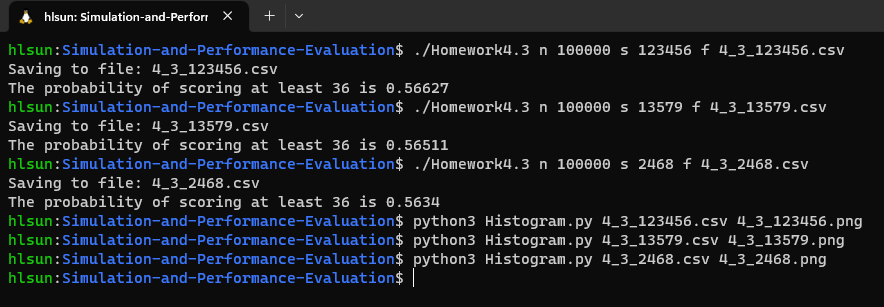
\includegraphics[scale=0.6]{Sections/Q3/4_3_terminal.png}\\
\newpage
Seed: 2468\\
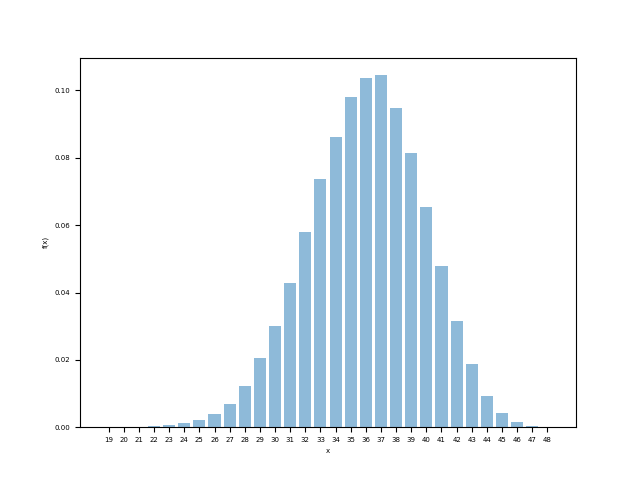
\includegraphics[scale=1]{Sections/Q3/4_3_2468.png}\\
\newpage
Seed: 13579\\
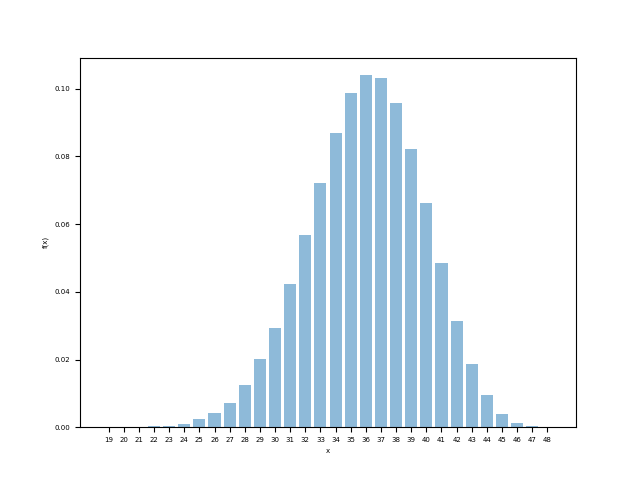
\includegraphics[scale=1]{Sections/Q3/4_3_13579.png}\\
\newpage
Seed: 123456\\
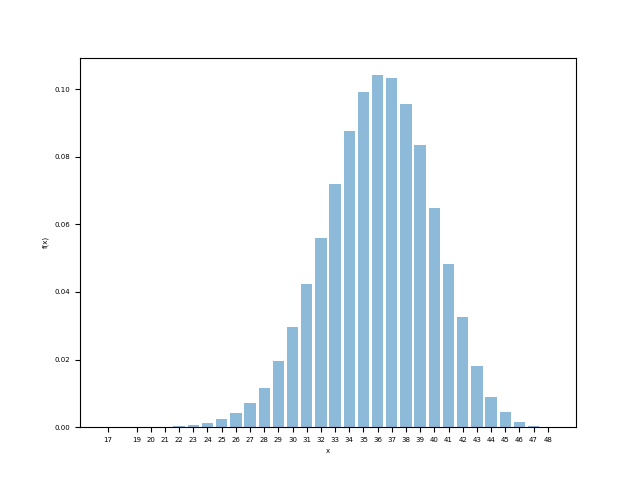
\includegraphics[scale=1]{Sections/Q3/4_3_123456.png}\\
\newpage

\begin{lstlisting}[style=CStyle]
/**
 * Harrison Sun (sun.har@northeastern.edu)
 * EECE 5643 - Simulation and Performance Evaluation
 * Homework 4.3
 */

#define DEFAULT_SEED 	    12345
#define DEFAULT_N_RUNS      100000
#define DEFAULT_PASSING		36
#define DEFAULT_OFILE		"output.txt"

// Define the grade weights
#define WEIGHT_A			4
#define WEIGHT_B			3
#define WEIGHT_C			2
#define WEIGHT_D			1
#define WEIGHT_F			0

#include <cstdlib>
#include <cstring>
#include <fstream>
#include <stdio.h>
#include <exception>
#include <iostream>
#include <list>
#include <math.h> 
#include <string>
#include <vector>
#include "c_lib/rvgs.h"
#include "c_lib/rngs.h"
#include "checkarg/checkarg.h"

/**
 * int weight
 * 
 * @param int n - The grade decision
 * @param int A - The weight of A
 * @param int B - The weight of B
 * @param int C - The weight of C
 * @param int D - The weight of D
 * @param int F - The weight of F
 * 
 * @return int grade - The weighted grade
 */

int weight(int n, int A, int B, int C, int D, int F) 
{
	int grade = 0;
	switch (n) {
	case 0:
		grade = A;
		break;
	case 1:
		grade = B;
		break;
	case 2:
		grade = C;
		break;
	case 3:
		grade = D;
		break;
	case 4:
		grade = F;
		break;
	}
	return grade;
}

 /**
  * int main() - The main function
  *
  * @param int argc - the number of arguments
  * @param char* argv[] - the arguments
  *
  * @return 0 if the program runs successfully
  */

int main(int argc, char* argv[])
{
	// There are 120 possible questions in the exam
	const int num_q{ 120 };
	// 90 Questions are classified as Class 1
	const int num_c1{ 90 };
	// 30 Questions are classified as Class 2
	const int num_c2{ 30 };
	// Doubly linked list to store the number of times each score is achieved <int score, long number of times scored>
	std::list<std::pair<int, long>> scoreCount;

    // Set the seed
    for (int i = 0; i < argc; ++i)
    {
        if (*argv[i] == 's' && checkArg(argv[i + 1]))
        {
            PutSeed(std::stol(argv[i + 1]));
            break;
        }
        else
        {
            PutSeed(DEFAULT_SEED);
        }
    }

	// Set the number of runs
	int nRuns{};
	for (int i = 0; i < argc; ++i)
	{
		if (*argv[i] == 'n' && checkArg(argv[i + 1]))
		{
			nRuns = std::stoi(argv[i + 1]);
			break;
		}
		else
		{
			nRuns = DEFAULT_N_RUNS;
		}
	}

	// Set the passing score
	int passingScore{};
	for (int i = 0; i < argc; ++i)
	{
		if (*argv[i] == 'p' && checkArg(argv[i + 1]))
		{
			passingScore = std::stoi(argv[i + 1]);
			break;
		}
		else
		{
			passingScore = DEFAULT_PASSING;
		}
	}

	// Set the grade weights
	int weightA{};
	int weightB{};
	int weightC{};
	int weightD{};
	int weightF{};
	
	for (int i = 0; i < argc; ++i)
	{
		if (*argv[i] == 'A' && checkArg(argv[i + 1]))
		{
			weightA = std::stoi(argv[i + 1]);
			break;
		}
		else
		{
			weightA = WEIGHT_A;
		}
	}

	for (int i = 0; i < argc; ++i)
	{
		if (*argv[i] == 'B' && checkArg(argv[i + 1]))
		{
			weightB = std::stoi(argv[i + 1]);
			break;
		}
		else
		{
			weightB = WEIGHT_B;
		}
	}
	
	for (int i = 0; i < argc; ++i)
	{
		if (*argv[i] == 'C' && checkArg(argv[i + 1]))
		{
			weightC = std::stoi(argv[i + 1]);
			break;
		}
		else
		{
			weightC = WEIGHT_C;
		}
	}

	for (int i = 0; i < argc; ++i)
	{
		if (*argv[i] == 'D' && checkArg(argv[i + 1]))
		{
			weightD = std::stoi(argv[i + 1]);
			break;
		}
		else
		{
			weightD = WEIGHT_D;
		}
	}

	for (int i = 0; i < argc; ++i)
	{
		if (*argv[i] == 'F' && checkArg(argv[i + 1]))
		{
			weightF = std::stoi(argv[i + 1]);
			break;
		}
		else
		{
			weightF = WEIGHT_F;
		}
	}

	// Set the filestream
	std::string outputFileName{};
	for (int i = 0; i < argc; ++i)
	{
		if (*argv[i] == 'f')
		{
			outputFileName = argv[i + 1];
			break;
		}
		else
		{
			outputFileName = DEFAULT_OFILE;
		}
	}

	// Class conditional probability
	const std::vector<double> class1Prob{ 0.6, 0.3, 0.1, 0.0, 0.0 };
	const std::vector<double> class2Prob{ 0.0, 0.1, 0.4, 0.4, 0.1 };


	// Run the simulation nRuns times
	for (int n = 0; n < nRuns; ++n)
	{
		// Reset the number of questions to the default
		int nq { num_q  };
		int nc1{ num_c1 };
		int nc2{ num_c2 };
		
		// Select 12 questions from the 120 questions without replacement
		// Determine the class and value of each question
		for (int i = 0; i < 12; ++i)
		{
			// Select a question
			int question = Equilikely(1, nq--); /* Note to self: nq-- is used here to decrement nq AFTER taking the Equilikely. --nq would not work the same way */
			// Determine the class of the question
			int questionClass = (question <= nc1) ? 1 : 2;
			// Determine the value of the question based on the class conditional probability and decrement the question class
			double random01 = Uniform(0, 1);
			// Store the cumulative value of the questions
			static int cumulativeValue{ 0 };
			
			if (questionClass == 1)
			{
				for (int j = 0; j < (int) class1Prob.size(); ++j)
				{
					if (random01 < class1Prob[j])
					{
						cumulativeValue += weight(j, weightA, weightB, weightC, weightD, weightF);
						break;
					}
					else
					{
						// This adjusts the randomly generated Uniform(0, 1) to account for rejecting the first comparison. The sum of the class conditional pdf is 1.0.
						random01 -= class1Prob[j];
					}
				}
				--nc1;
			}
			
			else	// (questionClass == 2)
			{
				for (int j = 0; j < (int) class2Prob.size(); ++j)
				{
				if (random01 < class2Prob[j])
					{
						cumulativeValue += weight(j, weightA, weightB, weightC, weightD, weightF);
						break;
					}
				else
					{
						// This adjusts the randomly generated Uniform(0, 1) to account for rejecting the first comparison. The sum of the class conditional pdf is 1.0.
						random01 -= class2Prob[j];
					}
				}
				--nc2;
			}
			// For the final question, store the score in scoreCount
			if (i == 11)
			{
				// Iterate through the linked list to find the correct scoreCount
				// If the score is not in the list, add it to the list and set the count to 1.
				// The score is sorted in ascending order.
				bool found = false;
				for (auto it = scoreCount.begin(); it != scoreCount.end(); ++it)
				{
					// The cumulativeValue is in the list
					if (it->first == cumulativeValue)
					{
						it->second++;
						found = true;
						break;
					}

					// The box is not in the list and a greater cumulativeValue value is found
					else if (it->first > cumulativeValue)
					{
						scoreCount.insert(it, std::make_pair(cumulativeValue, 1));
						found = true;
						break;
					}
				}
				// The cumulativeValue is not in the list and is greater than all cumulativeValues currently in the list
				if (!found)
				{
					scoreCount.push_back(std::make_pair(cumulativeValue, 1));
				}
				// Reset the cumulativeValue to 0 for the next run
				cumulativeValue = 0;
			} // End if (i == 11)
		} // End Question Selection
	}
	std::cout << "Saving to file: " << outputFileName << std::endl; /***************************************/
	// Store the contents of the linked list in csv format for plotting in Python
	std::ofstream outputFile;
	outputFile.open(outputFileName);
	for (auto it = scoreCount.begin(); it != scoreCount.end(); ++it)
	{
		outputFile << it->first << "," << (double) it->second / (double) nRuns << std::endl;
	}
	outputFile.close();

	// Determine whether pass or fail
	long passCount{ 0 };
	for (auto it = scoreCount.begin(); it != scoreCount.end(); ++it)
	{
		if (it->first >= passingScore)
		{
			passCount += it->second;
		}
	}
	
	std::cout << "The probability of scoring at least " << passingScore << " is " << (double) passCount / static_cast<double>(nRuns) << std::endl;
	return 0;
}
\end{lstlisting}